
%(BEGIN_QUESTION)
% Copyright 2006, Tony R. Kuphaldt, released under the Creative Commons Attribution License (v 1.0)
% This means you may do almost anything with this work of mine, so long as you give me proper credit

A liquid storage vessel uses a {\it bubbler} system to measure its liquid level:

$$\includegraphics[width=15.5cm]{i04159x01.eps}$$

Calculate the LRV and URV range points of the DP transmitter, in units of {\it kPa}:

\vskip 10pt

LRV = \underbar{\hskip 50pt}

\vskip 10pt

URV = \underbar{\hskip 50pt}

\vskip 10pt

\underbar{file i04159}
%(END_QUESTION)





%(BEGIN_ANSWER)

LRV = 9.87 kPa \hskip 50pt URV = 45.77 kPa

%(END_ANSWER)





%(BEGIN_NOTES)


%INDEX% Measurement, level: bubble tube (bubbler)
%INDEX% Measurement, level: dip tube
%INDEX% Measurement, level: hydrostatic pressure

%(END_NOTES)


